\chapter{知识库}
人类智能体通过学习和实践不断获取知识与经验,并能将习得的知识存储在记忆系统中,面对相关问题时能准确、快速地调用相关的知识和经验,完成识别和推理过程,成功解决问题。人工智能系统的终极目标便是能像人类一般快速、准确地解决未知问题,甚至超越人类的物理极限,实现范围更广、更艰深的任务解决。人类在真实世界中的学习是不断将非结构化的信息重构为结构化的知识的过程,知识库(KB)是一种包含常识和描述真实世界的事实的知识集,在不同的应用情景中有不同的内部结构。

\section{常见的知识库}
知识表达是人工智能中历史较为悠久的领域,并且大量的知识表达模型被提出,从最早的“框架和脚本”(frame and script)\citing{minsky1974framework,schank2013scripts}到后来的逻辑表达方式、资源描述框架(RDF)和网络本体语言(OWL)。随着互联网技术的普及,海量的网页、文章、超文本、图片等多种模态的资源被创造,如何将这些海量松散的多模数据重组为结构化的数据成为计算机科学的重要任务之一,大量的研究对信息的整合进行了探索\citing{smith1981multibase,wiederhold1993intelligent,subrahmanian1994amalgamating,embley1998ontology,alani2003automatic},语义网和相关技术的出现促进了大尺度知识库的发展,出现了DBpedia\citing{auer2007dbpedia}、OpenIE\citing{banko2007open}、Yago\citing{suchanek2007yago}、Freebase\citing{bollacker2008freebase}、Wikidata\citing{vrandevcic2014wikidata}等多种含有常识和特定领域知识的知识库。

除了知识库以外还有一种常用的存储数据的方式——数据库。数据库通常被组织成表格的方式,表内使用数值或者字符的方式表示数据,首行罗列出不同的属性,其余行则代表存储的数据。数据库中的表与表之间存在的指针代表表之间的联系。不同于数据库,知识库不以表为组织形式,而是由大量形式为(主语,谓语,宾语)的三元组构成的图结构,这样的三元组以资源描述框架(RDF)为模型基础\citing{lassila1997resource},能够方便的通过查询语句获得信息。“主语”和“宾语”表示知识库中的实体,“谓语”代表两者之间的关系。例如,将“猫种类属于哺乳类”转化的三元组形式为(猫,种类属于,哺乳类),“猫”是主语,“种类属于”是谓语,“哺乳类”是宾语。数据库与知识库的结构对比如图\ref{db-kb}。
\begin{figure}[H]
	\centering
	\subfigure[数据库的表结构]{
		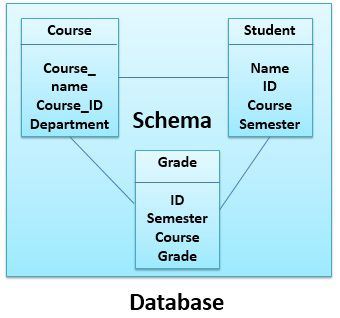
\includegraphics[width=0.5\textwidth]{database.jpg}}
	\subfigure[知识库的由三元组构成的图结构]{
		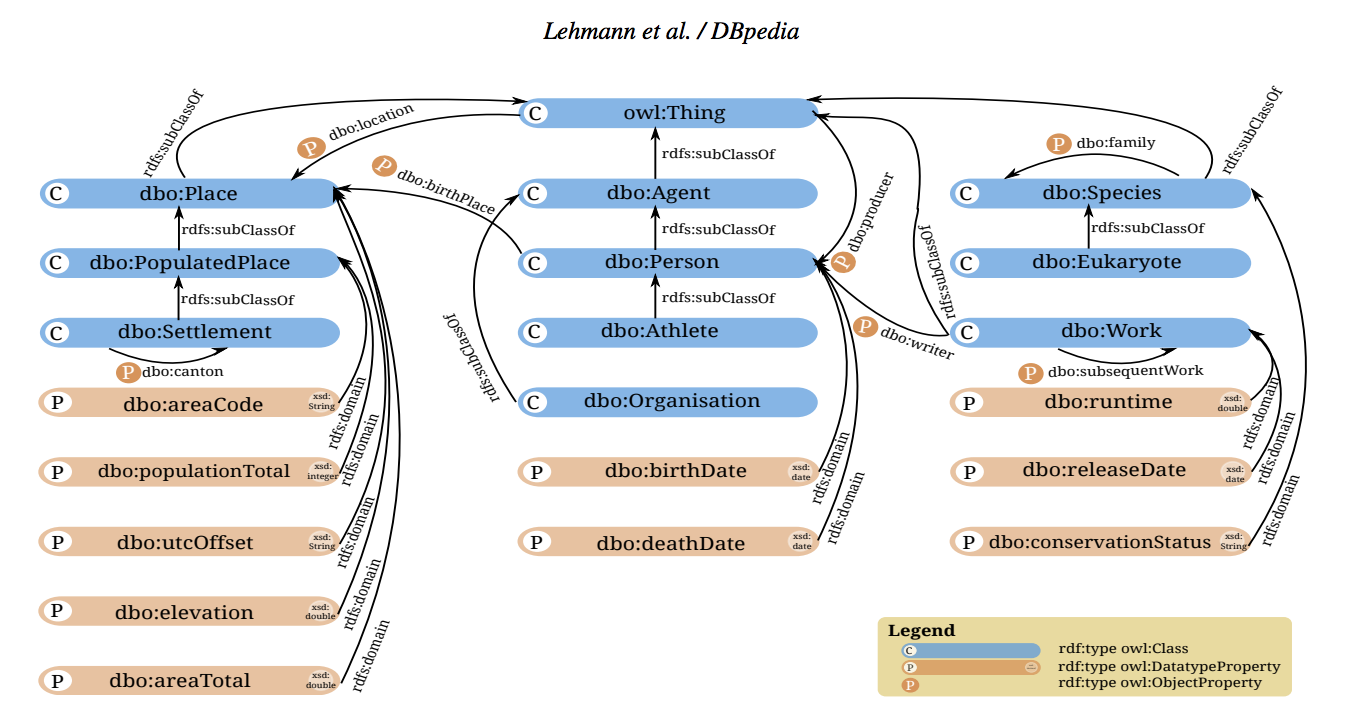
\includegraphics[width=0.7\textwidth]{kb.png}}
	\caption{数据库与知识库不同的数据组织形式}
	\label{db-kb}
\end{figure}

知识库具有高通用性、高可读性的特征。通过资源描述框架(RDF)能将所有现实中可描述的事物和事物间的关系组织到知识库中,这种通用性特征能够极大地提高了自动化系统存储、交换和使用信息;三元组的结构来源于语言学中“主谓宾”的基本语句构成方式,这既符合人类的认知方式,也是一种简单的数据组织形式,因此高可读性即使针对人类可读也是针对机器可读。正是因为知识库是建立在真实世界事实的描述之上,因此它能成为复杂决策和推理的基石,从人类推理过程看,知识库便是复杂推理的“起点”。

\subsection{Yago}
知识库通常由人工和自动化提取两种方式构建得到,对比这两种不同构建方式,自动化提取的知识库往往质量较低,容易包含错误信息,而人工构建的知识库能满足较高的精度要求,但由于人工构建的成本较高,因此此类知识库有数据容量受限、构建周期长、内容老化快等缺陷。

Suchanek等人结合Wikipedia文章的广博性和WordNet优秀的语义分类,提出了自动化生成本体的知识库YAGO\citing{suchanek2007yago}。Wikipedia的文章对某个话题或概念进行详细的多角度说明,同时大多数文章都归属于一个或者多个类别,类别页面既包含了大量实体和概念,可以作为知识库中的本体,同时类别页面也隐含着概念之间的平行关系和所属关系,这能提供一定的结构关系。YAGO利用Wikipedia目录页面提取出其中的实体和实体之间的关系,同时结合WordNet中概念的清晰层次关系,实现了97\%的准确率。初始版本中涉及90万个实体和500万个实体之间的关系。

YAGO被设计为可扩展的知识库,能够结合特定领域的知识源或是从网络上提取得到的信息构建领域相关的知识库,因此之后的研究者也在此基础上进行了多种的扩展。YAGO2在YAGO基础上引入GeoNames——包含超过700万个地点信息,在“实体-关联”的表示方法中加入了时间和空间维度,不仅能丰富事实的准确性,还能反应出实体在时空层面的变化\citing{hoffart2013yago2}。YAGO3构建了一个多语言的知识库\citing{mahdisoltani2013yago3}。

\subsection{DBpedia}
Wikipedia是由非盈利组织维基媒体基金会(Wikimedia Foundation)构建的世界上最大的多语言的开放性网络百科全书,其通过文章的形式对词条进行多方面的介绍,文章中包含大量的结构化信息,例如文字、信息框模板、分类信息、图片、地理坐标信息、超链接等,这些多模态的信息能丰富知识的多样性,并且建立知识的关联。但作为网络应用,Wikipedia的搜索能力和其他网络应用一样,只能满足关键词的搜索,这种状况大大的降低了知识之间的关联和价值,同时因为其作为大规模协同性内容编辑平台,文章内容也难以避免的出现数据矛盾、不一致的分类和错误。

Auer等人为了充分挖掘Wikipedia中已有的人类知识,并构建知识结构,提出了DBpedia知识库\citing{auer2007dbpedia}。Wikipedia为实现统一的文章风格,因此在文章编辑中镶嵌了一些信息框模板,如图\ref{dbpedia}。
\begin{figure}[h]
	\centering
	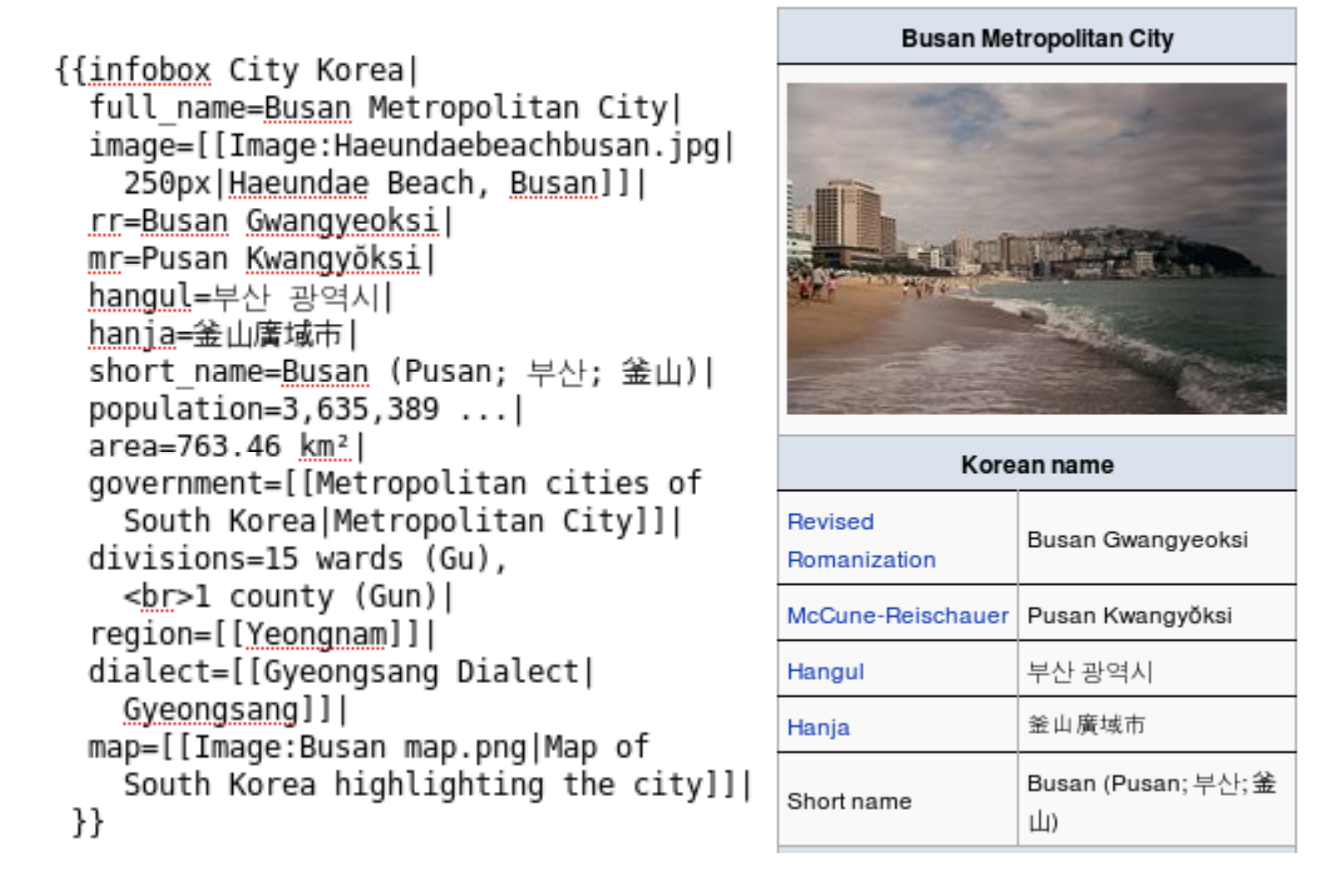
\includegraphics[width=0.8\textwidth]{dbpedia.png}
	\caption{Wikipedia的信息框模板和加载效果}
	\label{dbpedia}
\end{figure}
DBpedia利用信息框提取算法检测信息框模板,并且提取出关键的信息,再将信息转化为资源描述框架(RDF)的三元组结构,从而将Wikipedia的文章内容转化为机器可读的结构化信息。最初版本的DBpedia知识库包含关于195万实体的信息,实体内容包括人物、地点、音乐专辑和电影,除了实体外还包含65.7万个图片链接、160万个外部网页链接、18万个其他资源描述框架(RDF)数据库、20.7万个Wikipedia目录和7.5万个YAGO类别\citing{suchanek2007yago}。随着开放社区的数据丰富,2016年推出的版本中已经包含6600万实体,实体的类型扩充了视频、游戏、组织、物种和疾病\citing{wikipedia2016}。资源描述框架的三元组数据量也从1亿增长到130亿之多。

为了增强DBpedia的数据易用性,Auer等人提供了三种数据获取方式:链接数据、SPARQL协议和可下载的RDF文件。链接数据通过HTTP协议获取发布与互联网上的RDF数据,提供给语义网络浏览器、语义网路爬虫和语义网络查询客户端访问\citing{timlinked}。SPARQL是专门针对资源描述框架的查询语言,通过SPARQL终端向\url{http://dbpedia.org/sparql}发送查询指令,DBpedia知识库会返回相应的查询结果。可下载的RDF文件包含序列化的RDF三元组数据,DBpedia将整个数据库按照数据的类型分为众多子数据集,例如,文章目录集、目录标签集、地理坐标集、图像集等。

知识库的内容多样性、易用性和大体量为DBpedia应用提供了良好的基础设施,因此一些自然语言问答和交互的应用都选择建立在DBpedia丰富的知识之上。NLI-GO DBpedia是一个针对通用自然语言交互的应用程序,程序可以接受自然语言问题,并通过SPARQL查询DBpedia知识库,给出答案,实际上这就是基于DBpedia的文本问答系统\citing{nli-go},类似的还有款基于DBpedia的聊天机器人——DBpedia Chatbot。许多基于知识库的视觉问答研究也选择了数据更加准确的DBpedia\citing{wang2015explicit,wang2017fvqa,wu2016ask}。

\subsection{OpenIE}
应用于构建知识库的信息提取技术(IR)往往需要人为构建大量手写规则,并选择合适的语料库,当已有的提取模型面对全新领域的语料库时,需要重新编写提取规则或者标注数据,这种系统在面对快速迭代和具有丰富多样性的互联网数据时,便会遇到自动化程度低、语料库异质性和效率问题。

为了节省信息提取过程的自动化程度,并能大范围应用于不同领域,Banko等人提出了一种能自主学习不同语料库的信息提取模型——开放信息提取技术(Open IE)\citing{banko2007open}。Open IE以语料库为输入,通过内部算法对语料库中的语句进行一次遍历,最终提取出语句中蕴含的(实体,关系,实体)三元组数据,在整个过程中不需要人工参与,因此可以应用于不同领域知识库的构建。

Banko等人还提出了一种应用高扩展性Open IE模型的系统TEXTRUNNER。TEXTRUNNER由自监督学习器、单通道提取器、基于冗余的评估器三个主要模块构成。自监督学习器以小的语料样本作为训练集,首先使用语句解析器从样本中粗略地提取出(实体,关系,实体)的三元组数据,再对提取出的内容进行标注,标注为“可信”和“不可信”两种标签,将带有标签的数据作为朴素贝叶斯分类器的训练样本。提取器遍历整个语料库,提取出所有可能的三元组数据。对于同一个句子,提取器能生成一个或多个三元组数据,这些数据将被送入学习器训练得到的分类器中,保留所有分在“可信”类别的数据。在得到所有提取出的知识后,评估器融合相同的数据,计算不同的数据的数量。基于以上统计,评估器对每一个三元组数据分配一个用于判断知识正确性的概率值,其中的假设是,如果从多个的语句中提取出相同的知识,那么该知识拥有较高的可信度。

在实验阶段,TEXTRUNNER从包含1.3亿个句子的900万个网页中提取出6000万个三元组数据,平均每个句子提取出2.2个关系数据。通过数据过滤、随机抽取、人工判定等方式,作者对提取数据的完整性和正确性进行了概率评估,过滤后的数据包含1130万个三元组数据,其中780万的数据被评估为“格式正确”且概率标签在0.8以上,80.4\%“格式正确”的数据通过人工评估被认定为正确的,从实体间的关系看,“格式正确”的数据中反映抽象事实的占86\%,其中77.2\%是正确的;反映具体事实的占14\%,其中88.1\%是正确的,如图所示\ref{textrunner}。
\begin{figure}[H]
	\centering
	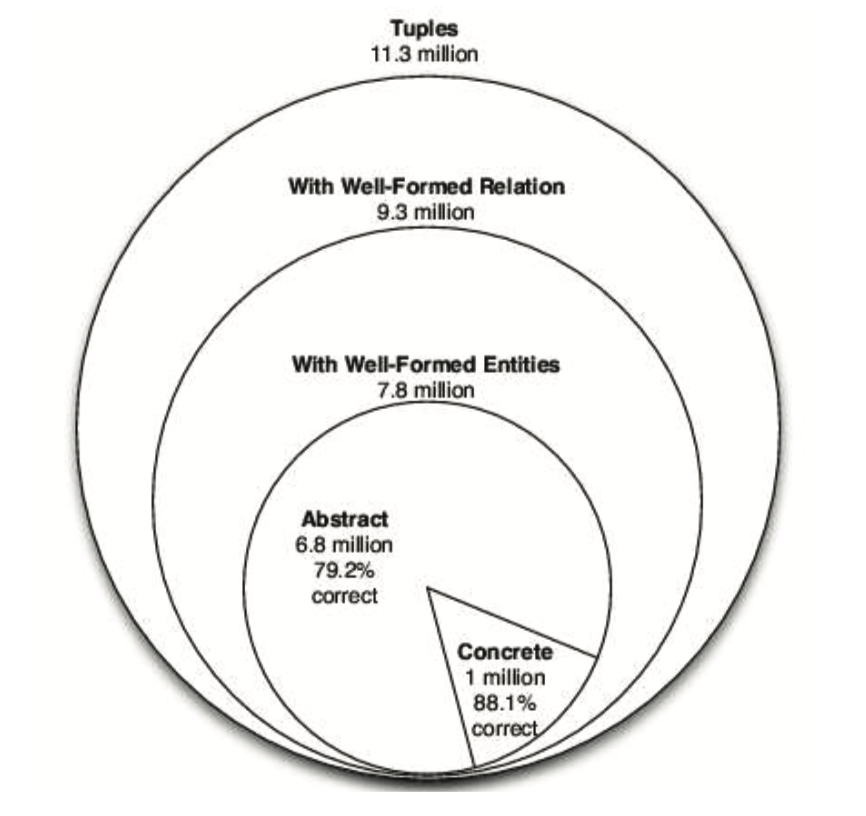
\includegraphics[width=0.5\textwidth]{textrunner.png}
	\caption{TEXTRUNNER在实验环境下知识提取的正确率}
	\label{textrunner}
\end{figure}

Wu等人在TEXTRUNNER的基础上提出了WOE开放信息提取系统\citing{wu2010open}。WOE改进了自监督学习方式用于构建提取器,TEXTRUNNER在提取过程中使用解析器直接从语料库中提取(实体,关系,实体)的三元组数据,而WOE则先从Wikipedia的信息框中提取“属性-值”对,再使用匹配器从文章中找到包含文章主语和“属性-值”对的句子作为语料库中的训练数据。随后测试了两种解析方法的提取器:WOE-parse和WOE-pos,WOE-pos使用和TEXTRUNNER类似的解析方法,根据简单的词性标签,从语料库中的句子解析出(实体,关系,实体)的数据,WOE-parse则选择更复杂的依赖解析树,希望能再复杂长句的解析中得到更好的精确度。

开放信息提取系统会对每个输出的三元组数据给定一个置信度,如果给定一个置信度的下限,高置信度的数据被保留,低置信度的数据被过滤,此时可以通过精确度和召回率测试系统的性能。精确度是指保留的数据中正确的数据所占比例,能反映整体精确度的平均水平。召回率是指保留的数据中正确的数据占所有正确数据的比例,能反映正确的数据在不同置信度的分布情况。

实验分析显示,因为使用了更友好的训练数据,WOE-pos在精确度上更优于TEXTRUNNER,而WOE-parse在解析树的帮助下实现了最好的性能,特别是在召回率上。

Fader等人在分析TEXTRUNNER和WOE的结果之后发现,不连贯提取和无信息提取两种错误频繁出现。不连贯提取是指被提取的关系语句由多词组成,但语义不连贯而无意义。无信息提取是指提取内容忽略了句子的关键信息,例如,“父亲对母亲做出承诺”,系统返回无信息的(父亲,做出,承诺)而不是(父亲,做出承诺对,母亲)。以上的两种错误都是由系统不能提取出具有完整句法结构的关系语句造成的,Fader等人在Open IE系统中引入了一定的句法限制,提出了REVERB开放信息提取系统\citing{fader2011identifying}。30\%的REVERB提取数据的概率标签在0.8或更高,相较起TEXTRUNNER的0.13\%,在精确度上实现了越阶式的增长,不连贯提取和无信息提取的错误率也大幅减少。

\subsection{Freebase}
Bollacker等人试图结合一般数据库的扩展和Wikipedia等百科全书的多样性,提出了Freebase数据库\citing{bollacker2008freebase}。Freebase和其他常用的知识库相同,使用资源描述框架的三元组形式结构化真实世界的知识,但同时继承了网络百科全书的开放和协同的思想,所有的内容创造和维护都由社区成员协作完成。Freebase存储的元组数据超过1亿2500万条,超过4000种类型和7000种属性,允许使用查询语言通过HTTP协议获取数据。

2014年,Google宣布关停Freebase并将数据迁移至Wikidata。

\subsection{Wikidata}
Wikidata是为了更高效地开放使用和管理Wikipedia文章中数据而提出的协同知识库\citing{vrandevcic2014wikidata}。由于Wikidata的出发点是希望通过大规模协同的方式构建知识库,因此Wikidata的数据具有开放性、多版本共存、多语言、易用性和持续更新的特性。Wikidata向所有用户提供数据扩展和编辑的权限;Wikidata为保证模糊数据的存疑性,相互之间有冲突的数据被同时展示;考虑到数字、日期、坐标等语言无关的数据内容,Wikidata与Wikipedia相同设计为多语言版本;Wikidata数据被组织成Json、RDF的形式发布于网络,通过网络服务能够轻松获取数据;社区成员的持续更新能保持Wikidata的时效性。

Wikidata数据的基本单元被称为项目(Item),每个项目包含名称标签、“Q+数字“的项目编码、描述、别名、和声明。声明中包含一系列属性和相应的值,用于详细描述项目的特点,项目页面如图\ref{wiki-item}。
\begin{figure}[H]
	\centering
	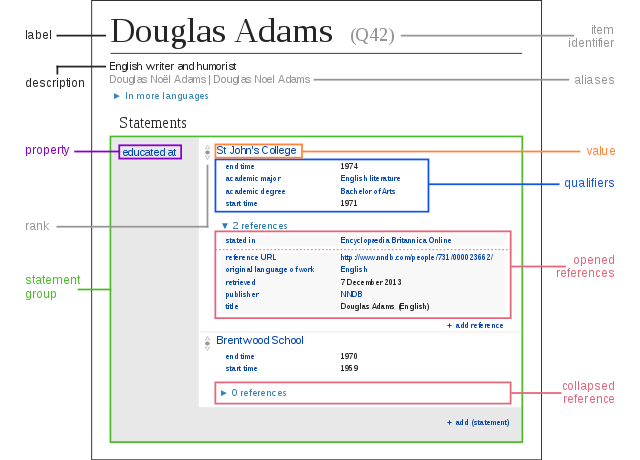
\includegraphics[width=0.8\textwidth]{wiki-item.png}
	\caption{wikidata项目页面}
	\label{wiki-item}
\end{figure}
项目之间通过有向无环图的方式构成,节点代表项目,有向线段代表项目之间的关系,如图\ref{wiki-dag}。截止到2018年,Wikidata已拥有超过5000万个项目。
\begin{figure}[H]
	\centering
	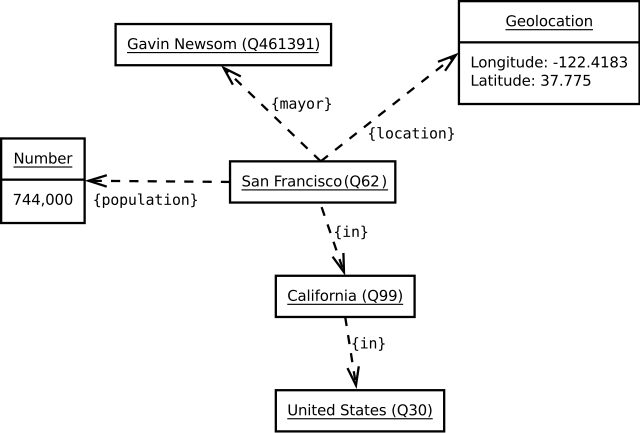
\includegraphics[width=0.8\textwidth]{wiki-dag.png}
	\caption{wikidata项目之间的有向无环图结构}
	\label{wiki-dag}
\end{figure}

Wikidata于2012年提出,相较起以往的知识库,开放性更强,限制也更少。对比YAGO和DBpedia,Wikidata不是从Wikipedia的目录或者信息框中提取信息,相反Wikidata被社区成员独立构建,并为Wikipedia作为知识源,数据被链接到Wikipedia文章中。对比Freebase将对象按类型划分的方式,Wikidata支持对所有对象赋予任意属性。

\section{知识库的应用}
知识库最早被应用于人工智能中的专家系统\citing{akerkar2010knowledge},专家系统是一种建立在知识库基础上,使用推理方法完成复杂推理过程,最终实现与人类专家同水平的决策能力的计算机系统,被广泛应用于医学诊断、分子结构推理、自然语言理解等领域。专家系统面向的专家任务需要特定领域的知识,这也使得知识库成为专家系统的核心之一。针对不同领域的任务构建知识的表达方式是困难的,因为专家知识可能是不精确的,同时要从知识库中获取答案的过程依赖于人工的制定复杂的规则,知识库精度和人力成本等因素制约了专家系统在更多领域的应用。

知识库也被应用于在自然语言处理的任务,例如机器翻译和文本问答。知识库中的本体包含某个领域中的各种概念和概念间的关系,本体在机器翻译中可作为知识源\citing{nirenburg1994machine}。语言学中的多义词在不同的语境中被解释为不同的含义,人类能根据上下文语境的不同选择出最恰当的词语,但对于机器翻译系统便是一大难题。当机器翻译系统能够获得足够多的本体作为知识源时,能较好地解决多义词的解释问题,从而得到更加准确的翻译结果\citing{knight1993building}。

文本问答系统在早期作为专家系统的交互界面,在之后的发展中逐渐独立出来成为自然语言处理的一个分支,文本问答系统根据给出的文本问题,从文本知识库中提取答案,此时的文本知识库往往是文本组成的文档,还未使用资源描述框架(RDF)的结构化数据。大多数文本问答系统都采用相对标准的结构:根据问题文本建立查询、利用信息提取方法(IR)确定可能包含答案的文章位置、进一步确定答案所在的片段,这种架构下不使用任何与答案相关的额外知识\citing{hermjakob2000knowledge}。Hermjakob等人提出了将手写规则和概念本体相结合的问答系统——Webclopedia\citing{hermjakob2000knowledge}。Webclopedia由对输入问题进行句法和语义的解析的问题解析模块、用于文档查询的查询模块、用于获得与答案相关的文档的信息提取模块、片段解析模块、答案匹配模块和答案生成模块构成。系统在多个模块中使用了知识库提高精确度,在问题解析过程中使用了语言知识库——由30000个节点的概念层级、140个问题/答案类型和词库组成,帮助系统确定问题的句法结构;在查询模块中使用了WordNet\citing{miller1995wordnet}扩展与问题关键词关联的信息;在答案匹配模块中也使用了常识和事实知识库,系统的架构如图\ref{Webclopedia}。
\begin{figure}[H]
	\centering
	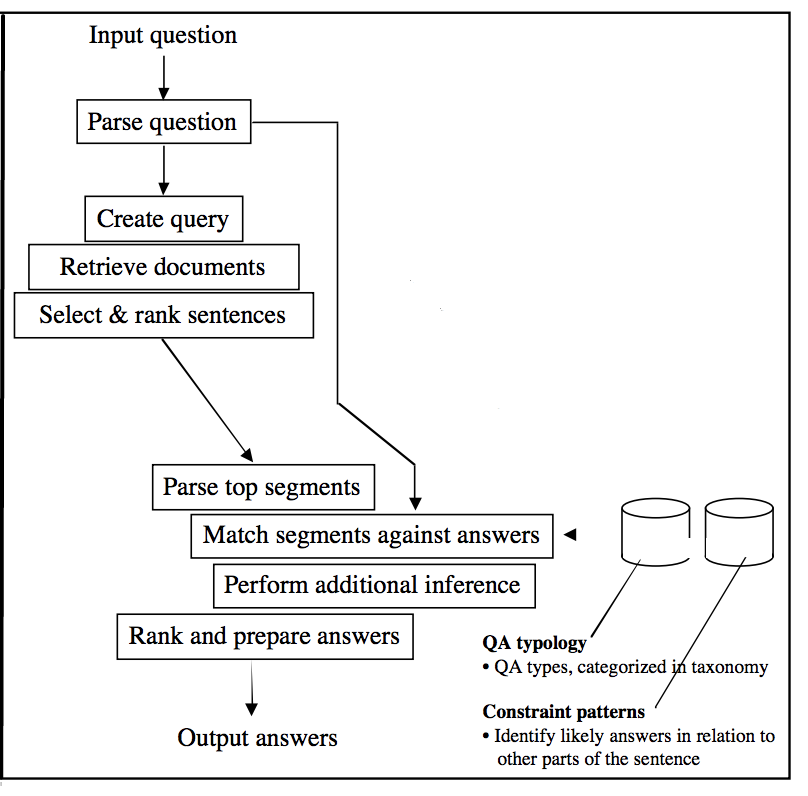
\includegraphics[width=0.8\textwidth]{Webclopedia.png}
	\caption{Webclopedia系统架构}
	\label{Webclopedia}
\end{figure}

应用信息提取技术(IR)的问答系统有一个非常明显的缺点——只能根据问题确定答案相关的文章或者段落,不能给出更为直接的答案。为解决这种缺陷,研究人员探索了更多的方法。

Burke等人一改通常的从文章中提取答案的方式,先将被频繁问到的问题(FAQ)以“问题-答案”对的形式存储为知识库,再从新问题中寻找与知识库匹配程度最高的“问题-答案”对,进而获得答案\citing{burke1997question}。在此方法中最核心的步骤是对新旧问题之间的匹配,为了使匹配的问题之间的语义相似度最大,系统还使用了WordNet\citing{miller1995wordnet}的语义知识,WordNet能提供词语和其同义词集合、同义词集合之间的关系,因此能避免一些匹配过程中的歧义错误,提高匹配的准确度。这里以“匹配”为核心思想的算法最大的障碍是常见问题集的容量、深度和广度问题,因此通常对于范围较小的场景而言,才能实现较好的匹配准确度。Rinaldi等人提出一个专门针对技术领域的基于知识的问答系统ExtrAns\citing{rinaldi2002towards}。ExtrAns以技术手册为知识库,将问题文本和知识库都转化为一种称为“最小逻辑形式”(MLF)的语义表达,并通过逻辑证明提取出答案。

随着资源描述框架(RDF)在构建知识库的兴起,知识库也由原来的文档形式转化为冗余更小、可扩展性更强、易用性更强的结构化数据库,这也促进了基于知识库的视觉问答方法的兴起。

\section{基于知识库的视觉问答方法}
视觉问答任务基于图像场景回答问题,图像理解、问题理解和答案生成是实现准确的视觉问答系统的算法核心。图像理解、问题理解和答案生成三者又可以根据人类思考逻辑将其划分为两个逻辑层次,问题理解成为逻辑基点,图像理解和答案生成都根据问题的不同而采用适当的算法策略——注意力机制便是一种借助问题理解而实现计算效率更高的图像解析方法,答案生成中关心的答案类型和答案词组长度也需要依照问题的不同而选择。因此问题的解析过程对于视觉问答算法的准确性和计算成本都有很大的影响。

正如绪论中提及的,问题可以分为识别和推理两个大类,推理任务中既要求系统能准确识别图像中的对象,往往也会涉及图像中无法获取的先验知识。先验知识包括众所周知但不会显性呈现的常识和面对特定领域需要具备的专业知识,例如,判断路口是否可以通行时,涉及基本交通规则的常识,判断艺术品的作者这类专业问题时,需要借助与该艺术品相关的知识储备。

先验知识对视觉问答系统提出了更高的要求,这也揭露了主流的联合嵌入模型的缺陷:第一点,联合嵌入模型的答案生成来源于训练集中的问题和答案文本,这意味着训练集中包含的知识和文本内容是整个视觉问答系统的所有知识来源,因此对于测试集中涉及的全新概念或答案,系统根本无法得出正确的答案。不断扩充包含更多先验知识的训练集是提高精度的方式之一,但对于整个世界蕴含的不可计量的知识而言,这种方式是不实际的。第二点,联合嵌入模型要求网络本身能存储学习到的知识,目前网络的容量相较于需要学习的知识是严重不足的。第三点,神经网络海量参数和复杂网络连接带来的黑盒特性依然存在。对于识别和分类等问题而言,可解释性与高精确度相比,显得不那么重要,但是对于需要明确推理过程的问答系统而言,黑盒的不可解释性会降低提问者对系统的可信度,毕竟没人会轻易相信一个无法解释的答案。

一种可行的解决方案是将推理过程和知识学习分离,保留系统原有的图像理解和问题文本理解模块,在答案生成模块中引入外源知识库。可扩展的外源知识库可以解决网络容量的限制问题;知识库中结构化的数据可以作为推理过程的起点,知识库中的数据关联能为推理提供路径,形成逻辑链条,提高系统的可解释性。本节将对已有的基于知识库的视觉问答方法进行详细的介绍,分析各种方法的优势和存在的问题。

\subsection{Ahab}

Wang等人提出的Ahab视觉问答系统利用DBpedia作为知识库,实现对需要先验知识的问题的推理应答,即使问题中涉及不包含于图像中的概念\citing{wang2015explicit}。Ahab的主要思路为三点,第一点,将图像中的概念链接到知识库中相同的概念,形成从图像到知识库的映射,第二点,将自然语言的文本问题处理为知识库查询语句,实现从自然语言的句法和语义结构变换到相应的查询语句结构,第三点,将知识库的查询结果转换为自然语言表达。利用以上三点,Ahab可以不通过数据集训练获取知识,而使用自然语言到知识库的两次转化完成问答任务。

具体来说,为了建立图像概念到知识库实体之间的映射,首先检测图像包含的概念,再将提取出的图像概念和知识库实体建立链接。Ahab从图像中提取物体对象、图像场景和图像属性三种视觉概念,对象提取使用在MS COCO\citing{lin2014microsoft}和ImageNet\citing{deng2009imagenet}上预训练后的Fast-RCNN\citing{ren2015faster},能实现224种类型的对象识别;场景分类器使用预处理于MIT Places205\citing{zhou2014learning}数据集的VGG-16 CNN,理论上能实现对205种场景的识别,每张图片选取分数前三的场景标签;图像属性提取器使用预处理于ImageNet\citing{deng2009imagenet}和MS COCO\citing{lin2014microsoft}的VGG-16 CNN,每张图片选取分数前十的属性标签。所有提取出的图像信息都使用资源描述框架(RDF)的形式表示,例如,“图像中包含长颈鹿对象”被表示为(图像,包含,对象1),(对象1,名称,长颈鹿)。每个视觉概念则被直接链接到具有相同语义的知识库概念,如图所示\ref{linkingMathord}。
\begin{figure}[H]
	\centering
	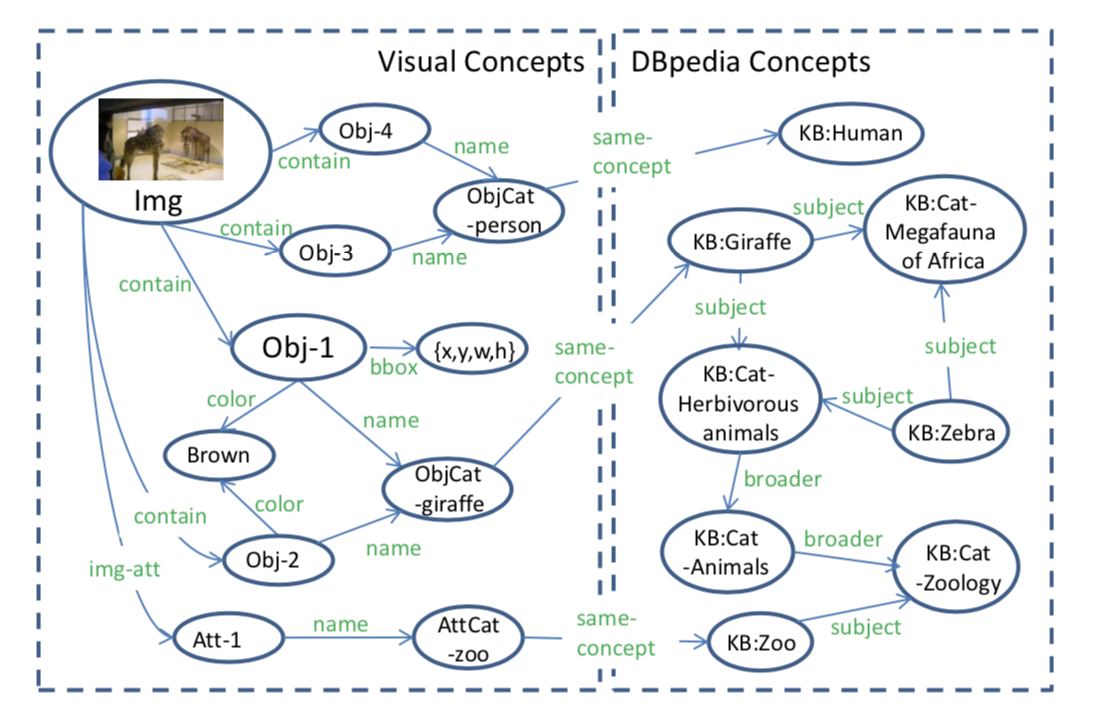
\includegraphics[width=0.8\textwidth]{linkingMathord.png}
	\caption{Ahab中链接图像信息和知识库实体的RDF图结构}
	\label{linkingMathord}
\end{figure}
所有资源描述框架(RDF)数据被存储在OpenLink Virtuoso中——一个能存储多种数据类型的数据库。

Ahab使用Quepy开源框架将自然语言问题转化为相应的知识库查询语句,但Quepy解析问题时,需要预先设定的正则表达式模板,因此Wang等人使用KB-VQA数据集作为实验数据集。结合KB-VQA中的23种问题模板和针对不同问题类型的谓语选择,Ahab能根据不同的问题产生相应的查询语句,并得到问题答案。

Ahab类似于专家系统,针对特定的问题设定了与之对应的知识库查询方法,应用于知识库的搜索路径可以为视为系统“逻辑推理”的过程,因此Ahab不仅输出最终的答案,而且也将答案推理的过程作为输出,实现了对系统推理的显性表达,问题处理的过程如图\ref{question_processing}。
\begin{figure}[H]
	\centering
	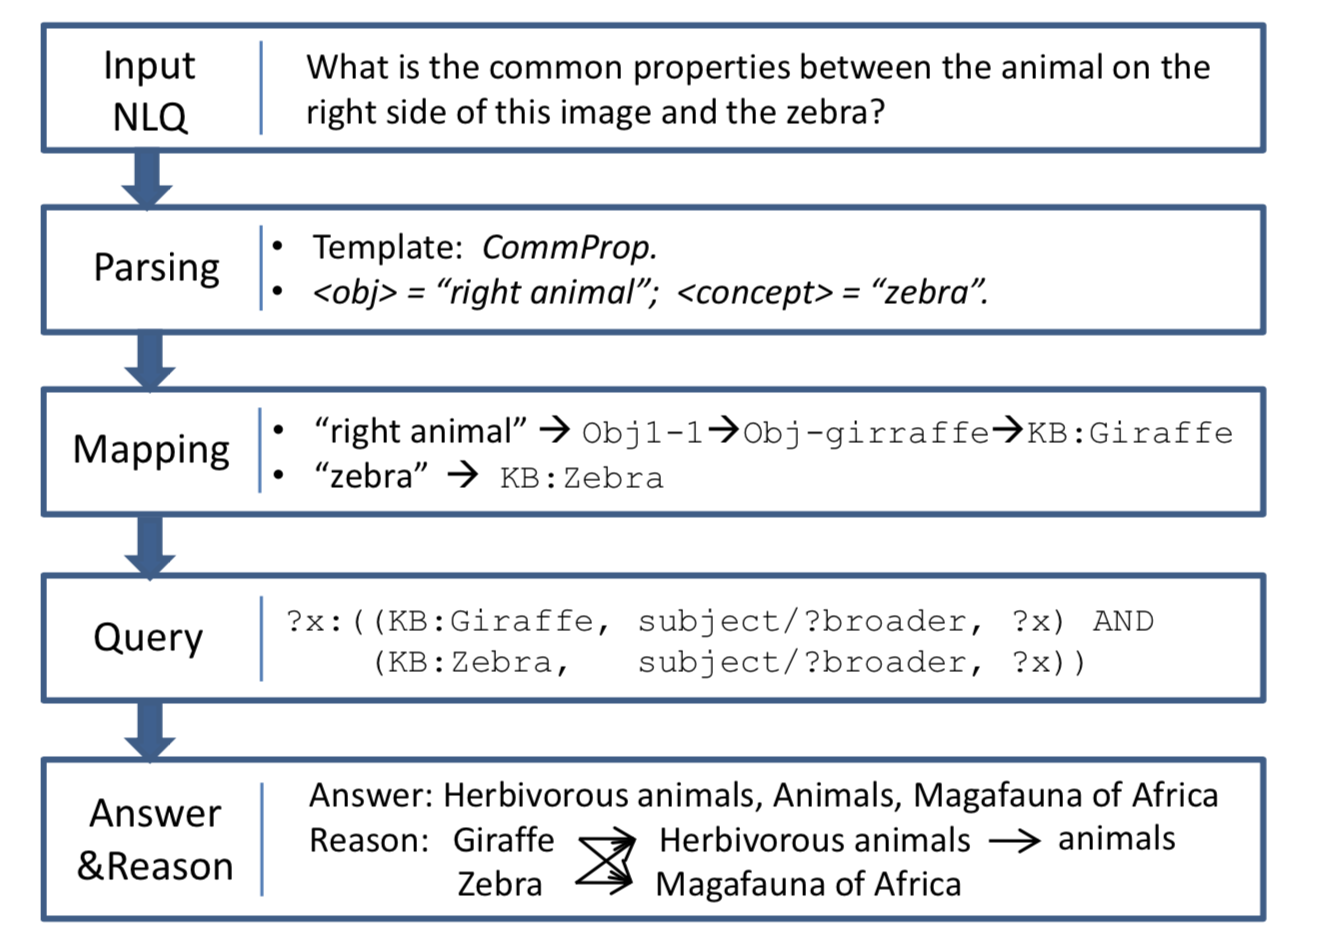
\includegraphics[width=0.8\textwidth]{question_processing.png}
	\caption{Ahab结合问题文本和预先设定的模板,解析出问题中的概念,再将问题中的概念与知识库实体建立链接,并生成查询语句,得到查询结果和推理过程}
	\label{question_processing}
\end{figure}

在评估Ahab对于需要先验知识的问题的表现时,Wang等人使用了自己构建的KB-VQA数据集(上文中有详细介绍)作为测试集,但KB-VQA中的问题多数是开放性的,并且还没有自动化评估正确性的方法被提出,因此使用人工的方式对结果的正确性进行评估,每个结果被人工地赋予5种表示正确程度的分数:1分-完全错误、2分-部分错误、3分-模棱两可、4分-基本正确、5分-完全正确。

作为对比,评估还引入了由人类作答和主流的联合嵌入模型作答两种方式——使用CNN编码图像特征,LSTM编码问题文本和生成答案的模型,三种测试系统在不同问题的正确率和平均得分如图\ref{ahab_evaluation}。
\begin{figure}[H]
	\centering
	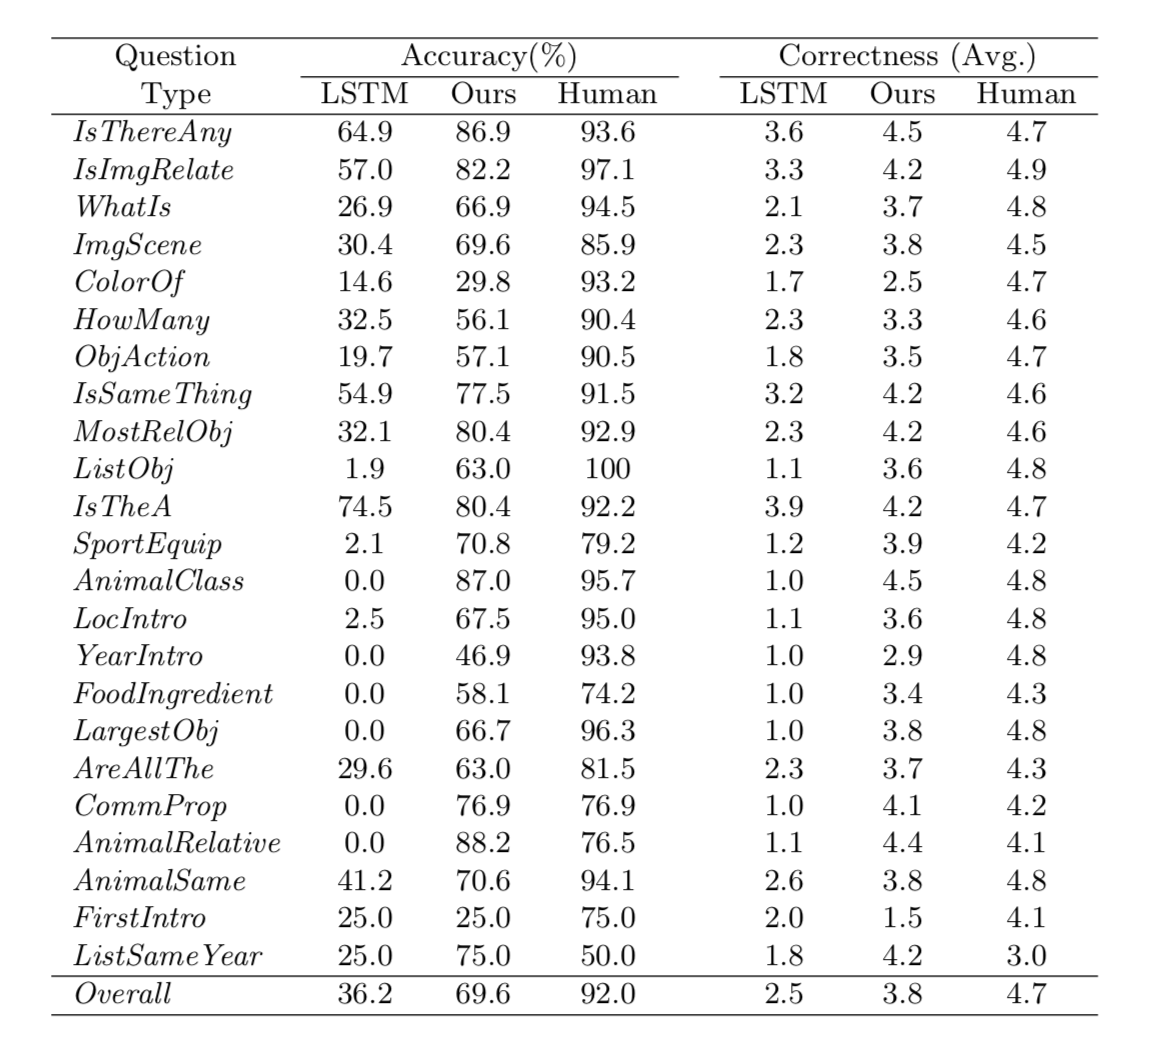
\includegraphics[width=0.8\textwidth]{ahab_evaluation.png}
	\caption{Ahab、联合嵌入模型和人类作答在23种问题上的表现。Accuracy是得分超过3的问题数量的比例,Correctness是某类问题得分的加权平均数。}
	\label{ahab_evaluation}
\end{figure}
KB-VQA将23种问题类型划分为“视觉问题”、“常识问题”、“知识库问题”三个知识等级,如图\ref{qtd},三种不同方法在三种知识等级的正确率统计如图\ref{type_evaluation}。
\begin{figure}[H]
	\centering
	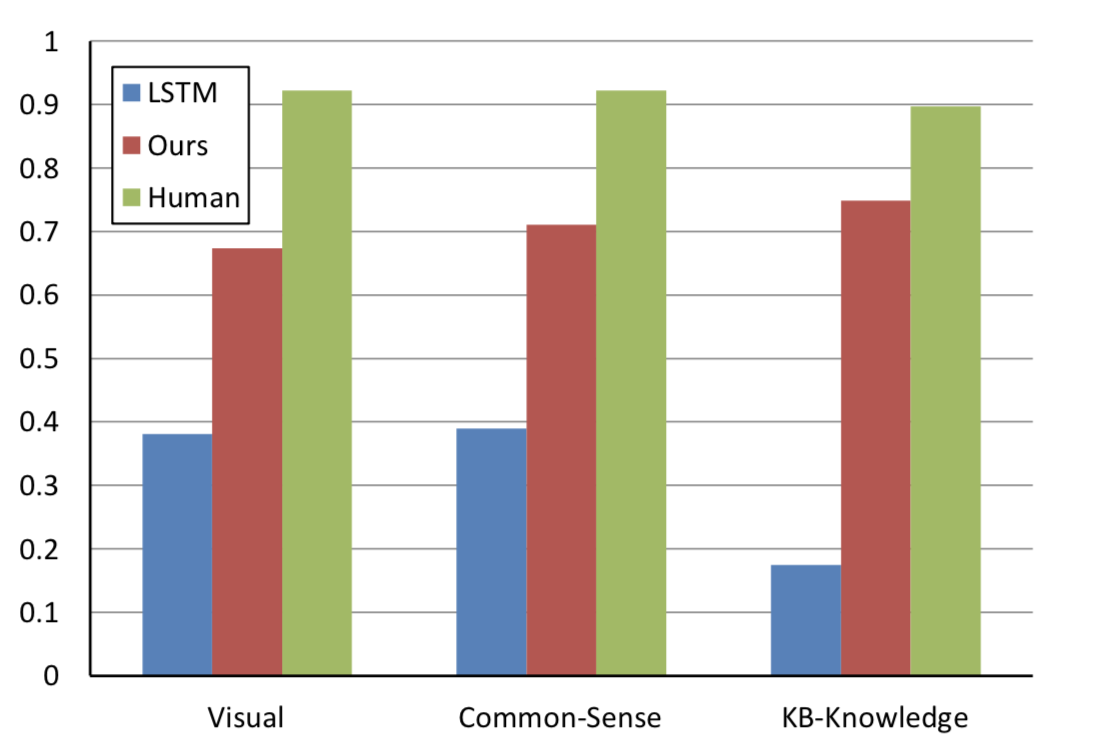
\includegraphics[width=0.8\textwidth]{type_evaluation.png}
	\caption{三种不同方法在三种知识等级的正确率统}
	\label{type_evaluation}
\end{figure}

从图\ref{qtd}中可以看出,LSTM的联合嵌入模型在“判断动物类别”、“判断对象生产年份”、“列出不同对象的共同属性”、“列出食物营养成分”、“判断最大/最小的物体”、“列出动物的近亲”这六种任务中正确率为0,其中除去“判断最大/最小的物体”为视觉问题外,其余5种问题均需要系统结合额外的知识回答,这正是基于训练集的概率模型的劣势——对于复杂关系和长知识链条的学习能力。总体上看,Ahab在每种问题类型上都优于联合嵌入模型,但离人类的正确率还是有一定差距,尤其在“判断物体颜色”和“比较两个物品的诞生先后”两种问题。

对于“列出与某个物品相同年份的物品”这类问题上,Ahab以75\%的准确率高出人类的50\%,但值得注意的是,KB-VQA数据集中此类问题只有4个,也就是说Ahab只是比人类多答对一个问题,考虑到答案生成过程和正确性评估过程中可能产生的误差,这并不能肯定的表明Ahab系统在此类问题上优于人类的表现。同样的状况也出现在其他问题类型上,因此KB-VQA在不同问题类型上数量的不均衡(问题数最多的类型与问题数最少的类型数量相差两个数量级)和问题样本数过小(16种问题类型的数量小于100,其中有两种的问题数量小于100)在评估视觉问答系统的真实推理能力上不能产生置信度足够高的结果,丰富数据集的样本和均衡不同类型的样本数量才能更好得评估系统的推理表现。

除了测试集存在稳定性较低和样本数较少的问题以外,Ahab系统只能针对预先设定的23种问题类型,这大大限制了问题的开放程度,不能满足真实的问答环境中海量的问题类型。而且Ahab的高正确率还建立在针对性地生成不同的问题查询语句之上,当问题类型数量剧增时,人工的对每种类型设定对应的算法是不切实际的,因此Ahab系统的扩展性也面临挑战。

但相较于主流使用统计方法的联合嵌入模型,Ahab利用知识库取代知识学习过程的方法在复杂推理任务,尤其是需要运用先验知识的问题上,实现了更好的系统表现,也为解决复杂推理问题的方法上提供了有益的实践。

\subsection{FVQA}
Ahab将问题解析为知识库查询语句时,需要预先确定问题模板,这极大的限制了系统面对多样化问题的能力,因此Wang等人改变了问题到查询语句的映射方式提出了FVQA模型\citing{wang2017fvqa}。FVQA模型使用带有FVQA数据集,FVQA数据集中的数据格式为(图片,问题,答案,支持事实),支持事实是一个包含答案的资源描述框架(RDF)数据,例如,(猫,能,爬树)。FVQA数据集中的问题包含三个属性:视觉概念(包含物体对象、场景和行为三种类型)、谓语(12种类型)和答案来源(图像和知识库两种)。FVQA模型在训练阶段,从标注后的支持事实中提取出问题的三种属性(VC表示视觉概念类型、REL表示谓语类型、AS表示知识来源类型),由于FVQA数据集中三种属性之间的组合能形成28类问题,所以FVQA模型使用长短期记忆(LSTM)网络训练一个28类的查询语句分类器,实现将问题到查询语句的分类过程,28种查询类型及其在训练/测试集的分布如图\ref{fvqa_query}。
\begin{figure}[H]
	\centering
	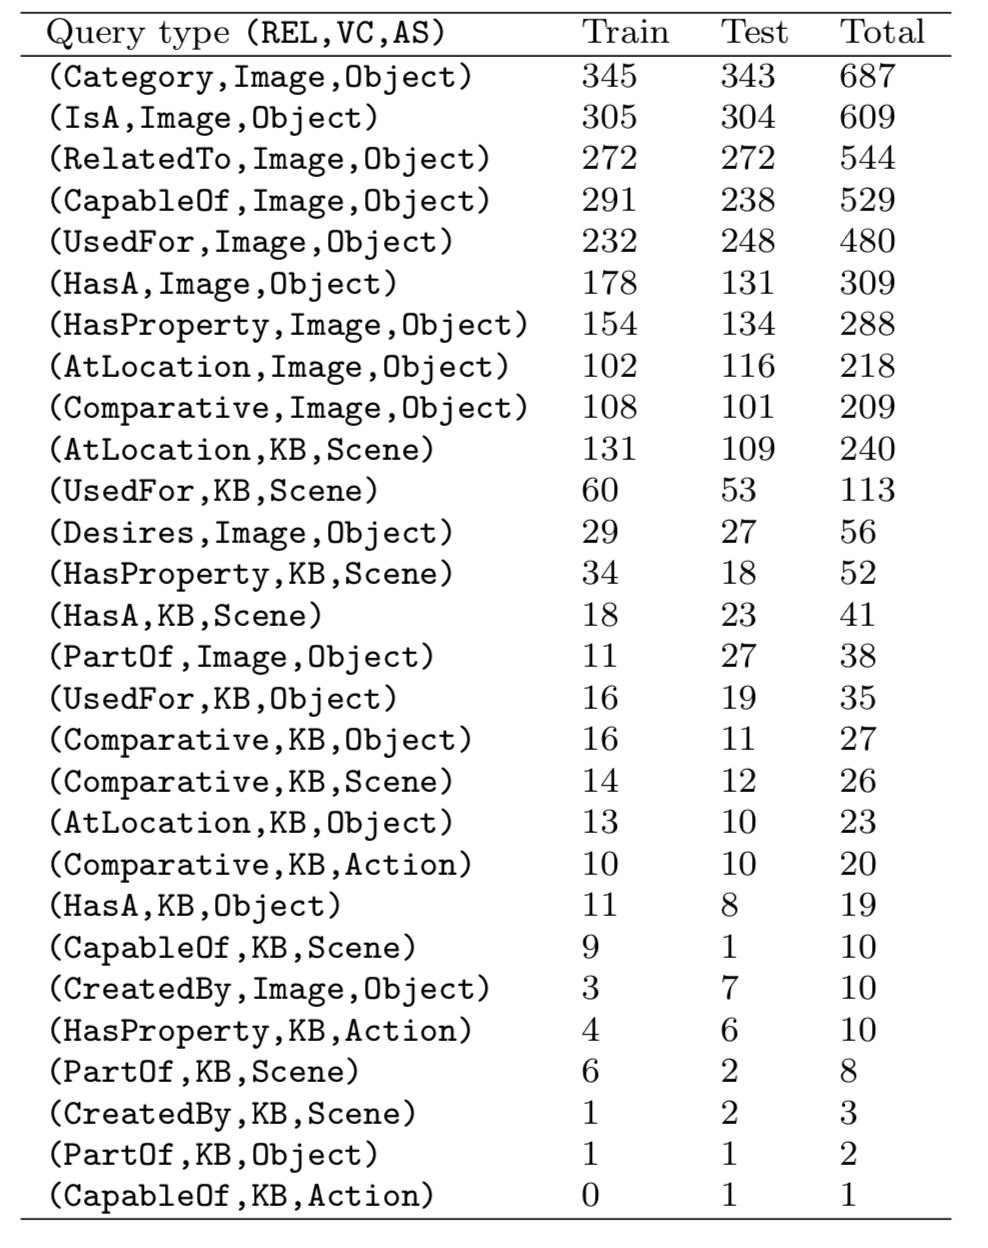
\includegraphics[width=0.5\textwidth]{fvqa_query.png}
	\caption{FVQA模型的28种查询类型及其在训练/测试集的分布情况}
	\label{fvqa_query}
\end{figure}

通过LSTM的分类,文本问题被映射为(REL,VC,AS)的查询类型,对于所有28种查询类型,查询语句都由下面的形式构成:
\begin{verbatim}
Find ?X, ?Y, subject to 
	{(ImgID,Contain,?X) and (?X,VC-Type,VC) and (?X,REL,?Y)}
\end{verbatim}
其中ImgID表示图片的标号,?X表示在图片ImgID中类型为VC的视觉概念,?Y表示在知识库中与?X通过谓语REL链接的概念。再根据AS是图片还是知识库的类型,使用不同的方法得到最终的答案。

FVQA模型中最核心的部分是将问题映射为对应的查询类型,图\ref{qqmaping}展示了问题到查询映射模型(QQmaping)在测试集中对应的三个知识库的正确率,可以看到映射模型在WebChild上实现了超过90\%的高正确率,但在其他两个知识库的准确率就相对较低,分析其中原因,可能是训练集和测试集中问题表达形式相似度的影响。WebChild中的谓语由图\ref{fvqa_vc}可知,都是两者比较的词汇,因此问题的表达形式较为单一,例如,“在图中什么物体更为<形容词的比较级>?”。
\begin{figure}[H]
	\centering
	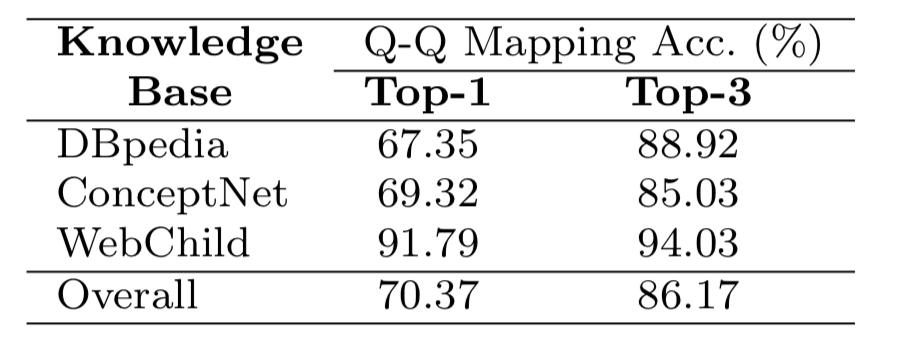
\includegraphics[width=0.5\textwidth]{qqmaping.png}
	\caption{问题到查询映射模型(QQmaping)在测试集中对应的三个知识库的正确率/测试集的分布情况}
	\label{qqmaping}
\end{figure}
引入支持向量机(SVM)\citing{chang2011libsvm}和使用长短期记忆(LSTM)的联合嵌入模型\citing{wu2016value}作为基线模型:只提供问题的SVM-Question和LSTM-Question、只提供图片的SVM-Image和LSTM-Image以及同时提供问题文本和图片的SVM-Question+Image和LSTM-Question+Image,各模型使用FVQA数据集作为训练和测试集中测试,不同模型的正确率见表\ref{fvqa_table}。
% Please add the following required packages to your document preamble:
% \usepackage{multirow}
% \usepackage[table,xcdraw]{xcolor}
% \usepackage{booktabs}
% If you use beamer only pass "xcolor=table" option, i.e. \documentclass[xcolor=table]{beamer}
\begin{table}[H]
% \resizebox{0.5\textwidth}{!}{}
\caption{不同模型在FVQA数据集上的测试正确率,Top-1表示只取得分最高的预测结果,Top-3和Top-10以此类推。灰色数据表示使用与问题对应的完全正确的查询类型时的正确率。}
\begin{tabular}{lccc}
\toprule
\multicolumn{1}{c}{} & \multicolumn{3}{c}{Overall Acc. (\%)}\\
\cmidrule(r){2-4}
\multicolumn{1}{c}{\multirow{-2}{*}{\textbf{Method}}} & \textbf{Top-1}& \textbf{Top-3} & \textbf{Top-10} \\
\midrule
SVM-Qusetion        & 11.19 & 20.68 & 32.14 \\
SVM-Image           & 17.55 & 30.75 & 49.02 \\
SVM-Qusetion+Image  & 17.99 & 31.83 & 49.55 \\
LSTM-Question       & 10.30 & 18.26 & 31.02 \\
LSTM-Image          & 22.69 & 36.21 & 58.59 \\
LSTM-Question+Image & 23.37 & 37.02 & 52.51 \\
\midrule
\cellcolor[HTML]{C0C0C0}gt-QQmaping & \cellcolor[HTML]{C0C0C0}64.23 & \cellcolor[HTML]{C0C0C0}71.58 & \cellcolor[HTML]{C0C0C0}72.74 \\
top-1-gt-QQmaping & 53.63 & 60.70 & 61.59 \\ 
top-3-gt-QQmaping & \textbf{58.19} & \textbf{65.89} & \textbf{66.83} \\
\bottomrule
\end{tabular}
\label{fvqa_table} 
\end{table}

从表\ref{fvqa_table}中Top-1一列可以看出,无论是SVM-Question+Image与SVM-Image之间的正确率差距还是LSTM-Question+Image与LSTM-Image的正确率差值都非常小,这说明问题的解析对于SVM和LSTM这两种模型正确率的提升没有太大的帮助,而两个模型总体的正确率也处于较低的水平,说明统计方法在样本较小的语料库中很难学习到知识间真正的逻辑关联。而FVQA模型使用问题到查询映射模型能从问题文本中提取到关键信息,并能利用关键信息组成有意义的语言结构,再结合额外知识库搜索到正确答案,答案获得的过程反映了推理的过程。gt-QQmaping(灰色背景)使用问题对应的正确查询类型,因此正确率反映了理想状况下FVQA模型从查询类型到生成查询语句过程中的误差情况,知识库查询过程的错误率在30\%左右。top-1-gt-QQmaping与gt-QQmaping之间的差距则代表问题到查询类型70.37\%(见图\ref{qqmaping})的正确率在最终答案的影响,top-3-gt-QQmaping的准确率高于top-1-gt-QQmaping的原因在是因为前者拥有更高的问题到查询类型映射的准确率。

表\ref{fvqa_answerSource}提供了不同方法在不同答案来源上的正确率,对比表中Image和KB两列容易看出,答案来源于视觉概念的准确率在所有模型上均远高于知识库来源,这说明表中涉及的三种模型都只能从图像和问题文本中包含的概念中提取答案,一旦答案涉及都额外知识库中的“新”概念,准确率便急剧下降,即使是使用额外知识库的gt-QQmaping。
\begin{table}[H]
% \resizebox{0.8\textwidth}{!}{}
\centering
\caption{不同方法在不同答案来源上的正确率}
\begin{tabular}{lcccccc}
\toprule
\multicolumn{1}{c}{\multirow{3}{*}{\textbf{Method}}} & \multicolumn{6}{c}{Answer-Source}\\
\cmidrule(r){2-7}
 & \multicolumn{3}{c}{\textbf{Image}} & \multicolumn{3}{c}{\textbf{KB}}\\
\cmidrule(r){2-4}
\cmidrule(r){5-7}
 & \textbf{Top-1} & \textbf{Top-3} & \textbf{Top-10} & \textbf{Top-1} & \textbf{Top-3} & \textbf{Top-10} \\
 \midrule
SVM-Qusetion        & 12.80 & 24.53 & 36.48 & 0.68 & 2.03 & 3.72 \\
SVM-Image           & 19.92 & 34.88 & 55.11 & 2.03 & 3.72 & 9.12 \\
SVM-Qusetion+Image  & 20.43 & 36.07 & 55.73 & 2.03 & 4.05 & 9.12 \\
LSTM-Question       & 11.71 & 20.49 & 34.21 & 1.01 & 3.72 & 10.14 \\
LSTM-Image          & 25.49 & 40.40 & 65.12 & 4.39 & 8.78 & 15.88 \\
LSTM-Question+Image & 26.01 & 41.12 & 58.05 & 6.08 & 10.14 & 16.22 \\
\midrule
\cellcolor[HTML]{C0C0C0}gt-QQmaping & \cellcolor[HTML]{C0C0C0}72.65 & \cellcolor[HTML]{C0C0C0}80.13 & \cellcolor[HTML]{C0C0C0}80.13  & \cellcolor[HTML]{C0C0C0}9.12 & \cellcolor[HTML]{C0C0C0}15.54 & \cellcolor[HTML]{C0C0C0}24.32 \\
top-1-gt-QQmaping & 60.89 & 68.27 & 68.27 & 6.08 & 11.15 & 17.91 \\ 
top-3-gt-QQmaping & \textbf{66.10} & \textbf{74.15} & \textbf{74.15} & \textbf{6.42} & \textbf{11.82} & \textbf{18.92} \\
\bottomrule
\end{tabular}
\label{fvqa_answerSource}
\end{table}

FVQA模型提出了一种以句法结构中的谓语为核心的先验知识问题的解答思路,首先从问题中解析出关键的谓语信息,在问题到查询类型模型中,结合谓语、视觉概念和答案来源决定了28种不同的查询类型,再使用生成的查询语句搜索基于12种谓语构建的知识库,最终预测答案。“主语-谓语-宾语”的一般句式结构中谓语表示了主语和宾语之间的相互作用,即使在相同的主语和宾语情况下,不同的谓语能表达出截然不同的语义信息,而绝大多数问题也能够直接通过谓语,推断答案的范畴。以谓语为基础的优势有几点,第一,易于问题分类。问题的自然语言表达方式众多,但无论如何改变句式结构,表达相同含义的谓语有限,通过对谓语的语义划分能够划分出问题的不同类型。第二,便于知识库的查询。知识库中的实体之间通过不同的谓语连接,形成错综复杂的知识网络,一个实体有众多连接,但一个谓语只连接两个实体,且往往谓语的两端就是问题的答案。

FVQA模型的缺陷有三点,第一,分类数量的确定和分类模型的精度。FVQA模型由于查询语句的生成依赖于查询类型,因此问题到查询类型映射的准确性会直接影响到答案生成的正确率。表\ref{fvqa_table}是在FVQA数据集上进行的,由于数据集中问题的类型只有28种,因此FVQA模型在问题到查询类型映射模型中使用了28类的分类器,但在实际问答环境中问题类型的具体数量远远多于28种,且无法预先确定,想训练能应用于实际情景中的FVQA模型不仅需要数据集的扩充,还需要提高模型本身的分类精度。第二,不能回答以谓语为答案的问题。所有28种查询类型都要求能从问题中提取关键谓语,并且所有答案都是物体对象,如果问题询问对象之间的关系,模型则无法从问题文本中获得谓语,不能得到答案。第三,不能很好的处理含有多个动词的复杂推理问题。FVQA模型的查询语句过于简单,仅仅将一次查询结果作为答案,在面对需要多级推理的问题时,便无法直接得到答案,如表\ref{fvqa_wrong}。
\begin{table}[H]
% \resizebox{0.8\textwidth}{!}{}
\centering
\begin{tabular}{lcccccc}
\toprule
\multicolumn{2}{c}{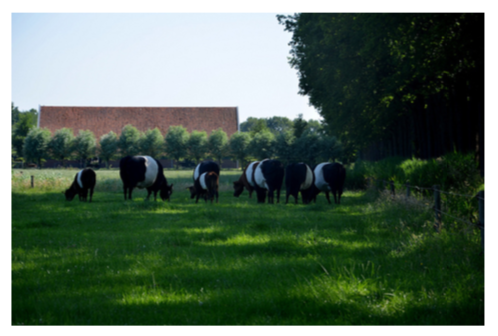
\includegraphics{cow.png}} \\
\multicolumn{2}{c}{What is related to the animal that can be found in this place?} \\
\midrule
\multirow{2}{*}{Mined Facet:} & You are likely to find a cow in a picture \\
 & The cow is related to the tree \\
Predicted Answer: & cow \\
Ground Truth: & tree \\
\bottomrule
\end{tabular}
\caption{问题中包含related和found两个动词,FVQA模型只能提取一个作为谓语并查询,选择found为谓语时,会出现错误的预测}
\label{fvqa_wrong}
\end{table}

\section{基于知识库的通用嵌入模型}
无论是Ahab还是FVQA模型都是通过将问题固定在一定类型,再通过对应不同问题的类型的额外知识库查询,获得更丰富的知识,从而提高复杂问题的正确率。为了提高视觉问答系统的问题的灵活性,Wu等人又通过改进常见的CNN+LSTM的嵌入模型,提出了基于知识库的通用嵌入模型。模型的基本架构由图像属性提取网络(CNN)、图像描述生成网络、外部知识库查询网络以及答案生成网络(LSTM)构成,模型架构如图\ref{KBLSTM}。
\begin{figure}[H]
	\centering
	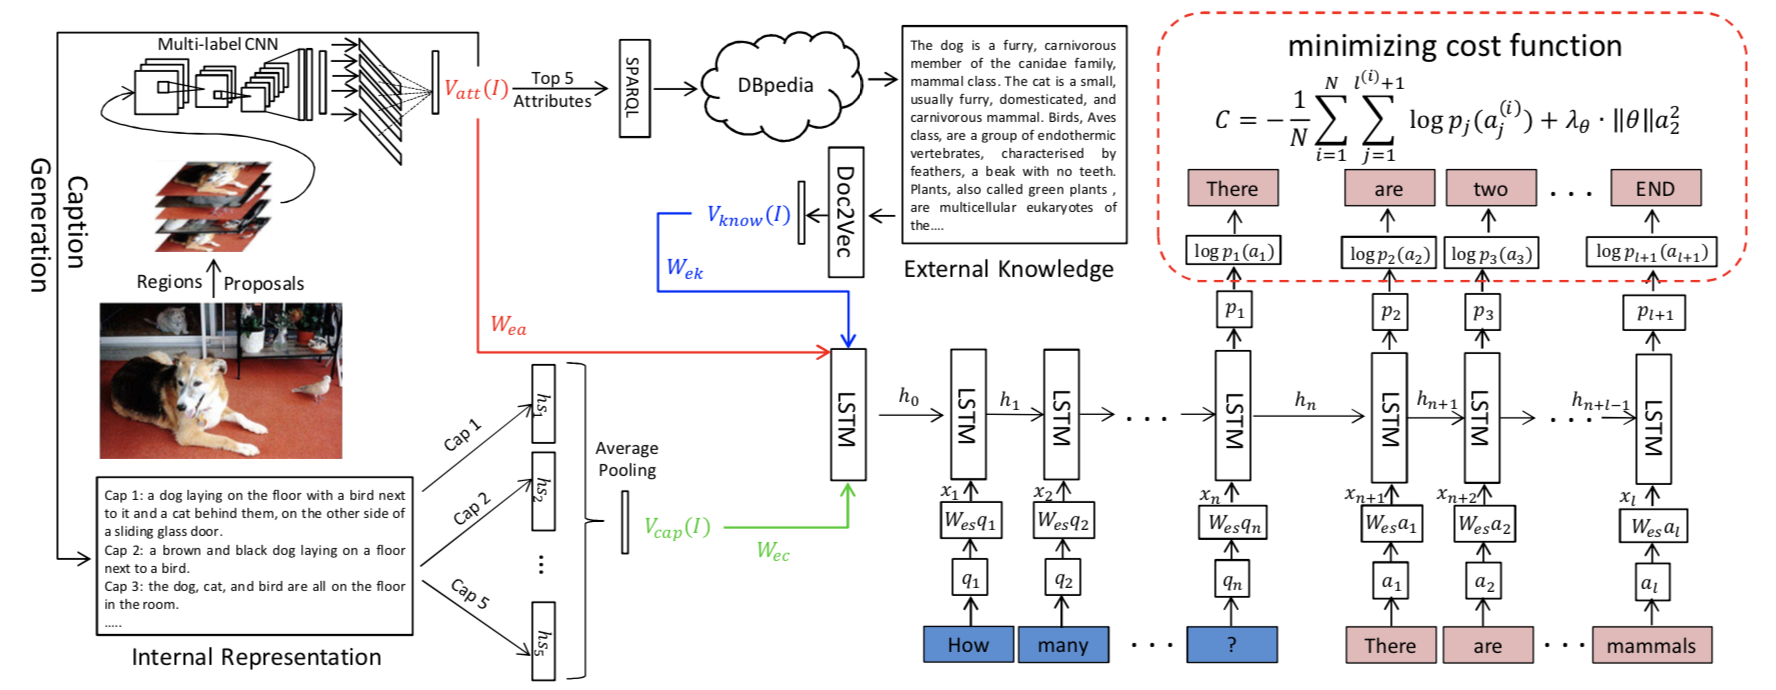
\includegraphics[width=0.8\textwidth]{KBLSTM.png}
	\caption{结合外部知识库的通用嵌入模型}
	\label{KBLSTM}
\end{figure}

图像属性提取网络将图像属性提取问题视为多标签的分类问题,以图像的多个子区域作为输入,输出前五个从MS COCO中筛选得到的图像属性$V_{att}(I)$,属性可能为物体名称、动作或者描述特征的形容词。提取出的图像属性分别作为图像描述生成网络和外部知识库查询网络的输入,图像描述生成网络将\cite{wu2016value}中的高层次的属性表达输入LSTM网络生成基于图像属性的描述,再将文本描述转化为五个特征向量,平均池化所有向量得到向量$V_{cap}(I)$。外部知识库查询网络首先分别将五个图像属性转化为知识库查询语言,查询到DBpedia知识库中相应的对象后,返回其“comment”——“comment”往往包含关于知识库对象最重要的解释信息,如图\ref{SPAQLexample},为了将大段的“comment”转化为向量,Wu等人使用Doc2Vec\citing{le2014distributed}——一种能方便的将句子、段落甚至文章等不固定长度的文本转化为固定大小的向量的模型,并且能包含文本内容的语义信息。——将其转化为$V_{know}(I)$。最后将$V_{att}(I)$、$V_{cap}(I)$、$V_{know}(I)$以及问题文本作为答案生成网络(LSTM)的输入,训练网络生成答案。
\begin{figure}[H]
	\centering
	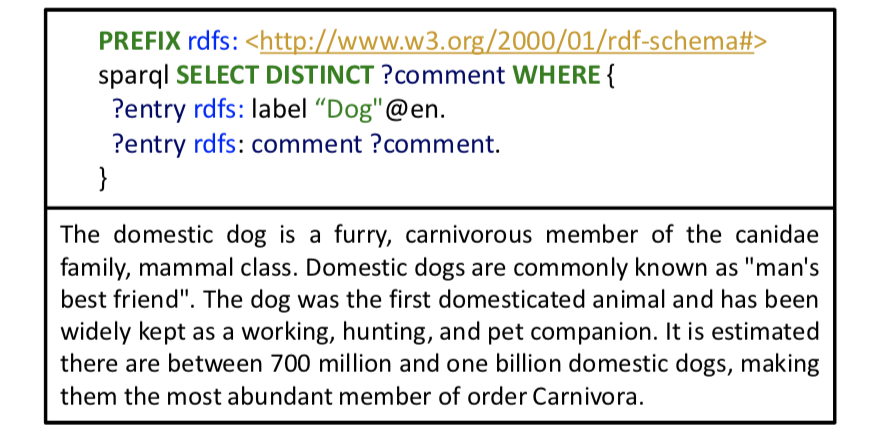
\includegraphics[width=0.5\textwidth]{SPAQLexample.png}
	\caption{使用‘dog’属性的查询语句以及返回的‘comment’内容}
	\label{SPAQLexample}
\end{figure}

在评估模型准确率时,由于该模型面对开放性问题,因此不同于Ahab和FVQA只能使用专门设计的数据集,该模型采用Toronto COCO-QA\citing{ren2015exploring}和VQA\citing{antol2015vqa}两个数据集进行评测。为了说明该模型的正确率情况,引入基线模型和几个结果较优的模型正确率作为对比,GUESS表示随机猜测模型,VggNet-LSTM使用在ImageNet上预处理的VggNet网络连接LSTM得到,VggNet+ft-LSTM使用在图像属性分类任务上微调后的VggNet,Att-LSTM表示直接将$V_{att}$作为LSTM输入的变体模型,类似的变体有Att+Cap-LSTM、Att+Know-LSTM、Att+Cap-LSTM、Cap+Know-LSTM,以及完整的Att+Cap+Know-LSTM模型。不同模型在两个数据集的正确率分别如表\ref{Wucoco}和\ref{Wuvqa}。
\begin{table}[H]
% \resizebox{0.8\textwidth}{!}{}
\centering
\caption{不同模型在Toronto COCO-QA正确率的表现}
\begin{tabular}{lc}
\toprule
\textbf{Toronto COCO-QA} & Acc(\%)\\
\midrule
GUESS\citing{ren2015image} & 6.65 \\
VggNet-LSTM & 50.73 \\
VggNet+ft-LSTM & 58.34 \\
\midrule
Att-LSTM & 61.38 \\
Att+Cap-LSTM & 69.02 \\
Att+Know-LSTM & 63.07 \\
Cap+Know-LSTM & 64.31 \\
\midrule
Att+Cap+Know-LS & \textbf{69.73} \\
\bottomrule
\end{tabular}
\label{Wucoco}
\end{table}

\begin{table}[H]
% \resizebox{0.8\textwidth}{!}{}
\centering
\caption{不同模型在VQA数据集的正确率表现}
\begin{tabular}{lc}
\toprule
\textbf{VQA} & Acc(\%)\\
\midrule
VggNet-LSTM & 44.93 \\
\midrule
Att-LSTM & 51.60 \\
Att+Cap-LSTM & 55.04 \\
Att+Know-LSTM & 53.79 \\
Cap+Know-LSTM & 52.31 \\
\midrule
Att+Cap+Know-LS & \textbf{55.96} \\
\bottomrule
\end{tabular}
\label{Wuvqa}
\end{table}
